% \documentclass[article]{standalone}
\documentclass[tikz]{standalone}

\usepackage{hyperref}
%\usepackage{hyperref, tikz}

% Determine flow chart stuff
\usetikzlibrary{shapes.geometric, arrows} % Arrows library
% Define block styles
%\tikzstyle{decision} = [diamond, draw, fill=blue!20, text width=4.5em, text badly centered, node distance=3cm, inner sep=0pt]
\tikzstyle{bblock} = [rectangle, draw, fill=blue!20, text width=11em, text centered, rounded corners, minimum height=4em, node distance = 7em]
\tikzstyle{yblock} = [rectangle, draw, fill=yellow!20, text width=11em, text centered, rounded corners, minimum height=4em, node distance = 7em]
\tikzstyle{rblock} = [rectangle, draw, fill=red!20, text width=11em, text centered, rounded corners, minimum height=4em, node distance = 7em]
\tikzstyle{wblock} = [rectangle, draw, fill=white, text width=11em, text centered, rounded corners, minimum height=4em, node distance = 7em]
\tikzstyle{secret} = [text width=1em, text centered, rounded corners, minimum height=1em, node distance = 2em]
\tikzstyle{line} = [draw, very thick, color=black, -latex']
\tikzstyle{rcloud} = [draw, ellipse, fill=red!20, text width=10em, node distance=5cm, minimum height=4em]
\tikzstyle{wcloud} = [draw, ellipse, fill=white, text width=10em, node distance=5cm, minimum height=4em]

%Change to sans serif font
\renewcommand{\familydefault}{\sfdefault}		%Alone with use Computer Modern sans serif
\usepackage{sansmathfonts}

\hypersetup{
    linktoc=all,     %set to all if you want both sections and subsections linked
}

\begin{document}

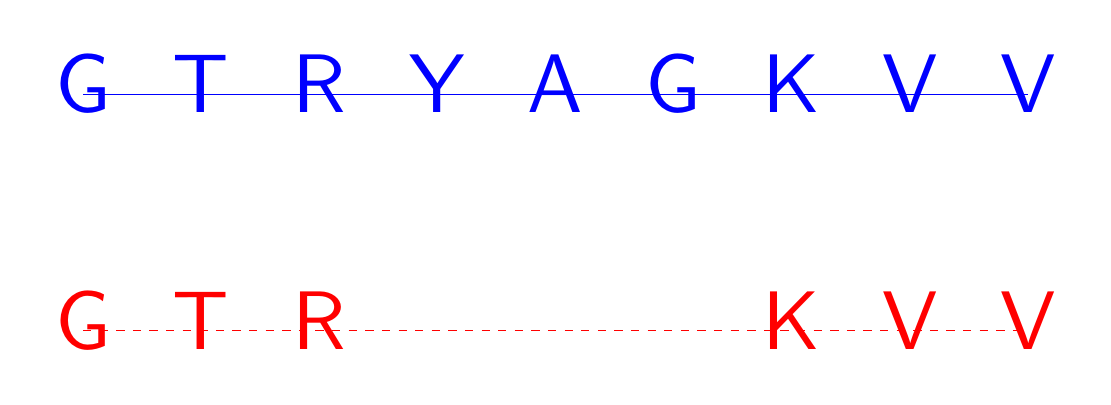
\begin{tikzpicture}[scale=3,transform shape]
  % Third, mid alignment
  \draw[anchor=mid, blue]    (0,1)  node{G} -- (0.5,1)  node{T} -- (1,1)  node{R} -- (1.5,1)  node{Y} -- (2,1)  node{A} -- (2.5,1)  node{G} -- (3,1)  node{K} -- (3.5,1)  node{V} -- (4,1)  node{V};
  \draw[anchor=mid, red, dashed]    (0,0)  node{G} -- (0.5,0)  node{T} -- (1,0)  node{R} -- (1.5,0)  node{} -- (2,0)  node{} -- (2.5,0)  node{} -- (3,0)  node{K} -- (3.5,0)  node{V} -- (4,0)  node{V};
\end{tikzpicture}

\end{document}
